% Options for packages loaded elsewhere
% Options for packages loaded elsewhere
\PassOptionsToPackage{unicode}{hyperref}
\PassOptionsToPackage{hyphens}{url}
\PassOptionsToPackage{dvipsnames,svgnames,x11names}{xcolor}
%
\documentclass[
  letterpaper,
  DIV=11,
  numbers=noendperiod]{scrartcl}
\usepackage{xcolor}
\usepackage{amsmath,amssymb}
\setcounter{secnumdepth}{-\maxdimen} % remove section numbering
\usepackage{iftex}
\ifPDFTeX
  \usepackage[T1]{fontenc}
  \usepackage[utf8]{inputenc}
  \usepackage{textcomp} % provide euro and other symbols
\else % if luatex or xetex
  \usepackage{unicode-math} % this also loads fontspec
  \defaultfontfeatures{Scale=MatchLowercase}
  \defaultfontfeatures[\rmfamily]{Ligatures=TeX,Scale=1}
\fi
\usepackage{lmodern}
\ifPDFTeX\else
  % xetex/luatex font selection
\fi
% Use upquote if available, for straight quotes in verbatim environments
\IfFileExists{upquote.sty}{\usepackage{upquote}}{}
\IfFileExists{microtype.sty}{% use microtype if available
  \usepackage[]{microtype}
  \UseMicrotypeSet[protrusion]{basicmath} % disable protrusion for tt fonts
}{}
\makeatletter
\@ifundefined{KOMAClassName}{% if non-KOMA class
  \IfFileExists{parskip.sty}{%
    \usepackage{parskip}
  }{% else
    \setlength{\parindent}{0pt}
    \setlength{\parskip}{6pt plus 2pt minus 1pt}}
}{% if KOMA class
  \KOMAoptions{parskip=half}}
\makeatother
% Make \paragraph and \subparagraph free-standing
\makeatletter
\ifx\paragraph\undefined\else
  \let\oldparagraph\paragraph
  \renewcommand{\paragraph}{
    \@ifstar
      \xxxParagraphStar
      \xxxParagraphNoStar
  }
  \newcommand{\xxxParagraphStar}[1]{\oldparagraph*{#1}\mbox{}}
  \newcommand{\xxxParagraphNoStar}[1]{\oldparagraph{#1}\mbox{}}
\fi
\ifx\subparagraph\undefined\else
  \let\oldsubparagraph\subparagraph
  \renewcommand{\subparagraph}{
    \@ifstar
      \xxxSubParagraphStar
      \xxxSubParagraphNoStar
  }
  \newcommand{\xxxSubParagraphStar}[1]{\oldsubparagraph*{#1}\mbox{}}
  \newcommand{\xxxSubParagraphNoStar}[1]{\oldsubparagraph{#1}\mbox{}}
\fi
\makeatother

\usepackage{color}
\usepackage{fancyvrb}
\newcommand{\VerbBar}{|}
\newcommand{\VERB}{\Verb[commandchars=\\\{\}]}
\DefineVerbatimEnvironment{Highlighting}{Verbatim}{commandchars=\\\{\}}
% Add ',fontsize=\small' for more characters per line
\usepackage{framed}
\definecolor{shadecolor}{RGB}{241,243,245}
\newenvironment{Shaded}{\begin{snugshade}}{\end{snugshade}}
\newcommand{\AlertTok}[1]{\textcolor[rgb]{0.68,0.00,0.00}{#1}}
\newcommand{\AnnotationTok}[1]{\textcolor[rgb]{0.37,0.37,0.37}{#1}}
\newcommand{\AttributeTok}[1]{\textcolor[rgb]{0.40,0.45,0.13}{#1}}
\newcommand{\BaseNTok}[1]{\textcolor[rgb]{0.68,0.00,0.00}{#1}}
\newcommand{\BuiltInTok}[1]{\textcolor[rgb]{0.00,0.23,0.31}{#1}}
\newcommand{\CharTok}[1]{\textcolor[rgb]{0.13,0.47,0.30}{#1}}
\newcommand{\CommentTok}[1]{\textcolor[rgb]{0.37,0.37,0.37}{#1}}
\newcommand{\CommentVarTok}[1]{\textcolor[rgb]{0.37,0.37,0.37}{\textit{#1}}}
\newcommand{\ConstantTok}[1]{\textcolor[rgb]{0.56,0.35,0.01}{#1}}
\newcommand{\ControlFlowTok}[1]{\textcolor[rgb]{0.00,0.23,0.31}{\textbf{#1}}}
\newcommand{\DataTypeTok}[1]{\textcolor[rgb]{0.68,0.00,0.00}{#1}}
\newcommand{\DecValTok}[1]{\textcolor[rgb]{0.68,0.00,0.00}{#1}}
\newcommand{\DocumentationTok}[1]{\textcolor[rgb]{0.37,0.37,0.37}{\textit{#1}}}
\newcommand{\ErrorTok}[1]{\textcolor[rgb]{0.68,0.00,0.00}{#1}}
\newcommand{\ExtensionTok}[1]{\textcolor[rgb]{0.00,0.23,0.31}{#1}}
\newcommand{\FloatTok}[1]{\textcolor[rgb]{0.68,0.00,0.00}{#1}}
\newcommand{\FunctionTok}[1]{\textcolor[rgb]{0.28,0.35,0.67}{#1}}
\newcommand{\ImportTok}[1]{\textcolor[rgb]{0.00,0.46,0.62}{#1}}
\newcommand{\InformationTok}[1]{\textcolor[rgb]{0.37,0.37,0.37}{#1}}
\newcommand{\KeywordTok}[1]{\textcolor[rgb]{0.00,0.23,0.31}{\textbf{#1}}}
\newcommand{\NormalTok}[1]{\textcolor[rgb]{0.00,0.23,0.31}{#1}}
\newcommand{\OperatorTok}[1]{\textcolor[rgb]{0.37,0.37,0.37}{#1}}
\newcommand{\OtherTok}[1]{\textcolor[rgb]{0.00,0.23,0.31}{#1}}
\newcommand{\PreprocessorTok}[1]{\textcolor[rgb]{0.68,0.00,0.00}{#1}}
\newcommand{\RegionMarkerTok}[1]{\textcolor[rgb]{0.00,0.23,0.31}{#1}}
\newcommand{\SpecialCharTok}[1]{\textcolor[rgb]{0.37,0.37,0.37}{#1}}
\newcommand{\SpecialStringTok}[1]{\textcolor[rgb]{0.13,0.47,0.30}{#1}}
\newcommand{\StringTok}[1]{\textcolor[rgb]{0.13,0.47,0.30}{#1}}
\newcommand{\VariableTok}[1]{\textcolor[rgb]{0.07,0.07,0.07}{#1}}
\newcommand{\VerbatimStringTok}[1]{\textcolor[rgb]{0.13,0.47,0.30}{#1}}
\newcommand{\WarningTok}[1]{\textcolor[rgb]{0.37,0.37,0.37}{\textit{#1}}}

\usepackage{longtable,booktabs,array}
\usepackage{calc} % for calculating minipage widths
% Correct order of tables after \paragraph or \subparagraph
\usepackage{etoolbox}
\makeatletter
\patchcmd\longtable{\par}{\if@noskipsec\mbox{}\fi\par}{}{}
\makeatother
% Allow footnotes in longtable head/foot
\IfFileExists{footnotehyper.sty}{\usepackage{footnotehyper}}{\usepackage{footnote}}
\makesavenoteenv{longtable}
\usepackage{graphicx}
\makeatletter
\newsavebox\pandoc@box
\newcommand*\pandocbounded[1]{% scales image to fit in text height/width
  \sbox\pandoc@box{#1}%
  \Gscale@div\@tempa{\textheight}{\dimexpr\ht\pandoc@box+\dp\pandoc@box\relax}%
  \Gscale@div\@tempb{\linewidth}{\wd\pandoc@box}%
  \ifdim\@tempb\p@<\@tempa\p@\let\@tempa\@tempb\fi% select the smaller of both
  \ifdim\@tempa\p@<\p@\scalebox{\@tempa}{\usebox\pandoc@box}%
  \else\usebox{\pandoc@box}%
  \fi%
}
% Set default figure placement to htbp
\def\fps@figure{htbp}
\makeatother





\setlength{\emergencystretch}{3em} % prevent overfull lines

\providecommand{\tightlist}{%
  \setlength{\itemsep}{0pt}\setlength{\parskip}{0pt}}



 


\KOMAoption{captions}{tableheading}
\makeatletter
\@ifpackageloaded{caption}{}{\usepackage{caption}}
\AtBeginDocument{%
\ifdefined\contentsname
  \renewcommand*\contentsname{Table of contents}
\else
  \newcommand\contentsname{Table of contents}
\fi
\ifdefined\listfigurename
  \renewcommand*\listfigurename{List of Figures}
\else
  \newcommand\listfigurename{List of Figures}
\fi
\ifdefined\listtablename
  \renewcommand*\listtablename{List of Tables}
\else
  \newcommand\listtablename{List of Tables}
\fi
\ifdefined\figurename
  \renewcommand*\figurename{Figure}
\else
  \newcommand\figurename{Figure}
\fi
\ifdefined\tablename
  \renewcommand*\tablename{Table}
\else
  \newcommand\tablename{Table}
\fi
}
\@ifpackageloaded{float}{}{\usepackage{float}}
\floatstyle{ruled}
\@ifundefined{c@chapter}{\newfloat{codelisting}{h}{lop}}{\newfloat{codelisting}{h}{lop}[chapter]}
\floatname{codelisting}{Listing}
\newcommand*\listoflistings{\listof{codelisting}{List of Listings}}
\makeatother
\makeatletter
\makeatother
\makeatletter
\@ifpackageloaded{caption}{}{\usepackage{caption}}
\@ifpackageloaded{subcaption}{}{\usepackage{subcaption}}
\makeatother
\usepackage{bookmark}
\IfFileExists{xurl.sty}{\usepackage{xurl}}{} % add URL line breaks if available
\urlstyle{same}
\hypersetup{
  pdftitle={Class 7: Machine Learning 1},
  pdfauthor={Mayla (PID: A19136116)},
  colorlinks=true,
  linkcolor={blue},
  filecolor={Maroon},
  citecolor={Blue},
  urlcolor={Blue},
  pdfcreator={LaTeX via pandoc}}


\title{Class 7: Machine Learning 1}
\author{Mayla (PID: A19136116)}
\date{}
\begin{document}
\maketitle

\renewcommand*\contentsname{Table of contents}
{
\hypersetup{linkcolor=}
\setcounter{tocdepth}{3}
\tableofcontents
}

\subsection{Background}\label{background}

Today we will explore some core machine learning methods that are very
popular in bioinformatics. These include: \textbf{clustering} and
\textbf{dimensionality reduction}.

\subsection{K-means clustering}\label{k-means-clustering}

The main function in ``base'' R for K-means clustering, is called
\texttt{kmeans()}

Before we go too deep let's make up some ``simple'' data that we can
cluster and know if we are getting a good answer or not. To help us do
this, we can use \texttt{r}norm()` function:

\begin{Shaded}
\begin{Highlighting}[]
\FunctionTok{hist}\NormalTok{( }\FunctionTok{rnorm}\NormalTok{(}\DecValTok{1000}\NormalTok{, }\AttributeTok{mean =} \DecValTok{3}\NormalTok{) )}
\end{Highlighting}
\end{Shaded}

\pandocbounded{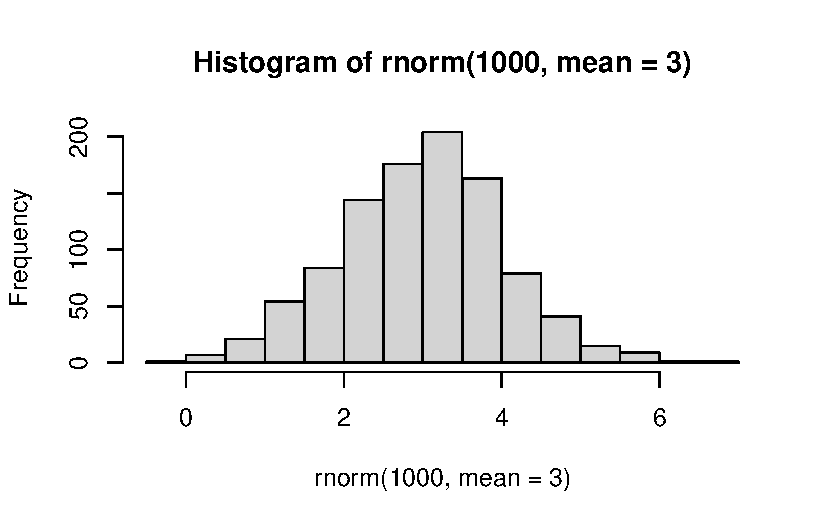
\includegraphics[keepaspectratio]{class07_files/figure-pdf/unnamed-chunk-1-1.pdf}}

\begin{Shaded}
\begin{Highlighting}[]
\NormalTok{x }\OtherTok{\textless{}{-}} \FunctionTok{c}\NormalTok{( }\FunctionTok{rnorm}\NormalTok{(}\DecValTok{30}\NormalTok{, }\AttributeTok{mean =} \SpecialCharTok{{-}}\DecValTok{3}\NormalTok{), }\FunctionTok{rnorm}\NormalTok{(}\DecValTok{30}\NormalTok{, }\AttributeTok{mean =} \SpecialCharTok{+}\DecValTok{3}\NormalTok{) )}
\end{Highlighting}
\end{Shaded}

\begin{Shaded}
\begin{Highlighting}[]
\NormalTok{z }\OtherTok{\textless{}{-}} \FunctionTok{cbind}\NormalTok{( }\AttributeTok{x =}\NormalTok{ x, }\AttributeTok{y =} \FunctionTok{rev}\NormalTok{(x) )}
\FunctionTok{plot}\NormalTok{(z)}
\end{Highlighting}
\end{Shaded}

\pandocbounded{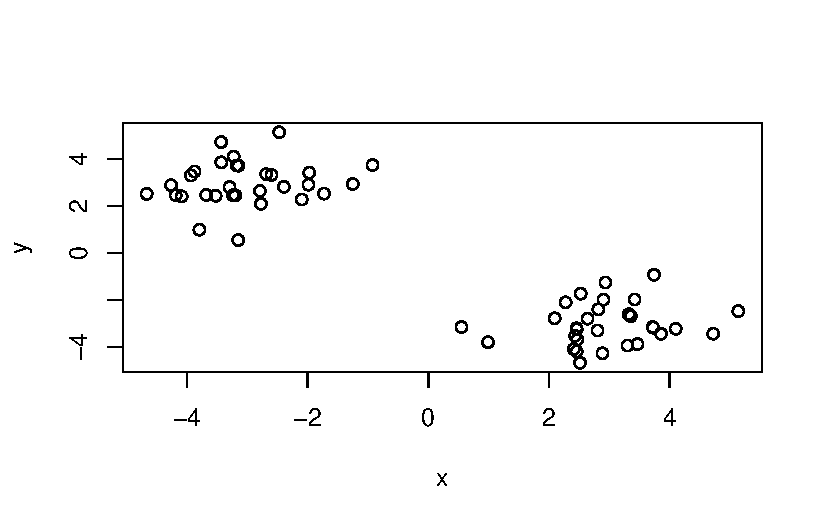
\includegraphics[keepaspectratio]{class07_files/figure-pdf/unnamed-chunk-3-1.pdf}}

\begin{Shaded}
\begin{Highlighting}[]
\CommentTok{\#cbind() / rbind() combibes by column/rows}
\end{Highlighting}
\end{Shaded}

\begin{Shaded}
\begin{Highlighting}[]
\NormalTok{p }\OtherTok{\textless{}{-}} \DecValTok{1}\SpecialCharTok{:}\DecValTok{5}

\FunctionTok{cbind}\NormalTok{(p,}\FunctionTok{rev}\NormalTok{(p))}
\end{Highlighting}
\end{Shaded}

\begin{verbatim}
     p  
[1,] 1 5
[2,] 2 4
[3,] 3 3
[4,] 4 2
[5,] 5 1
\end{verbatim}

\begin{Shaded}
\begin{Highlighting}[]
\FunctionTok{rbind}\NormalTok{(p,}\FunctionTok{rev}\NormalTok{(p))}
\end{Highlighting}
\end{Shaded}

\begin{verbatim}
  [,1] [,2] [,3] [,4] [,5]
p    1    2    3    4    5
     5    4    3    2    1
\end{verbatim}

Now we can run \texttt{kmeans(0)} on this input \texttt{z} and see what
the results look like.

\begin{Shaded}
\begin{Highlighting}[]
\NormalTok{km }\OtherTok{\textless{}{-}} \FunctionTok{kmeans}\NormalTok{(z, }\AttributeTok{centers =} \DecValTok{2}\NormalTok{)}
\NormalTok{km}
\end{Highlighting}
\end{Shaded}

\begin{verbatim}
K-means clustering with 2 clusters of sizes 30, 30

Cluster means:
          x         y
1  2.951190 -3.034294
2 -3.034294  2.951190

Clustering vector:
 [1] 2 2 2 2 2 2 2 2 2 2 2 2 2 2 2 2 2 2 2 2 2 2 2 2 2 2 2 2 2 2 1 1 1 1 1 1 1 1
[39] 1 1 1 1 1 1 1 1 1 1 1 1 1 1 1 1 1 1 1 1 1 1

Within cluster sum of squares by cluster:
[1] 49.16207 49.16207
 (between_SS / total_SS =  91.6 %)

Available components:

[1] "cluster"      "centers"      "totss"        "withinss"     "tot.withinss"
[6] "betweenss"    "size"         "iter"         "ifault"      
\end{verbatim}

\begin{Shaded}
\begin{Highlighting}[]
\FunctionTok{attributes}\NormalTok{(km)}
\end{Highlighting}
\end{Shaded}

\begin{verbatim}
$names
[1] "cluster"      "centers"      "totss"        "withinss"     "tot.withinss"
[6] "betweenss"    "size"         "iter"         "ifault"      

$class
[1] "kmeans"
\end{verbatim}

\begin{quote}
Q. How many points are in each cluster?
\end{quote}

\begin{Shaded}
\begin{Highlighting}[]
\NormalTok{km}\SpecialCharTok{$}\NormalTok{size}
\end{Highlighting}
\end{Shaded}

\begin{verbatim}
[1] 30 30
\end{verbatim}

\begin{quote}
Q. What ``component of your result object details cluster
assignment/membership?
\end{quote}

\begin{Shaded}
\begin{Highlighting}[]
\NormalTok{km}\SpecialCharTok{$}\NormalTok{cluster}
\end{Highlighting}
\end{Shaded}

\begin{verbatim}
 [1] 2 2 2 2 2 2 2 2 2 2 2 2 2 2 2 2 2 2 2 2 2 2 2 2 2 2 2 2 2 2 1 1 1 1 1 1 1 1
[39] 1 1 1 1 1 1 1 1 1 1 1 1 1 1 1 1 1 1 1 1 1 1
\end{verbatim}

\begin{quote}
Q. What ``component of your result object details cluster center?
\end{quote}

\begin{Shaded}
\begin{Highlighting}[]
\NormalTok{km}\SpecialCharTok{$}\NormalTok{centers}
\end{Highlighting}
\end{Shaded}

\begin{verbatim}
          x         y
1  2.951190 -3.034294
2 -3.034294  2.951190
\end{verbatim}

\begin{quote}
Q. Plot \texttt{z} colored by the kmeans cluster assignment and add
cluster centers as blue points.
\end{quote}

\begin{Shaded}
\begin{Highlighting}[]
\FunctionTok{plot}\NormalTok{(z, }\AttributeTok{col=}\NormalTok{km}\SpecialCharTok{$}\NormalTok{cluster)}
\FunctionTok{points}\NormalTok{(km}\SpecialCharTok{$}\NormalTok{centers, }\AttributeTok{col=} \StringTok{"blue"}\NormalTok{, }\AttributeTok{pch =} \DecValTok{15}\NormalTok{)}
\end{Highlighting}
\end{Shaded}

\pandocbounded{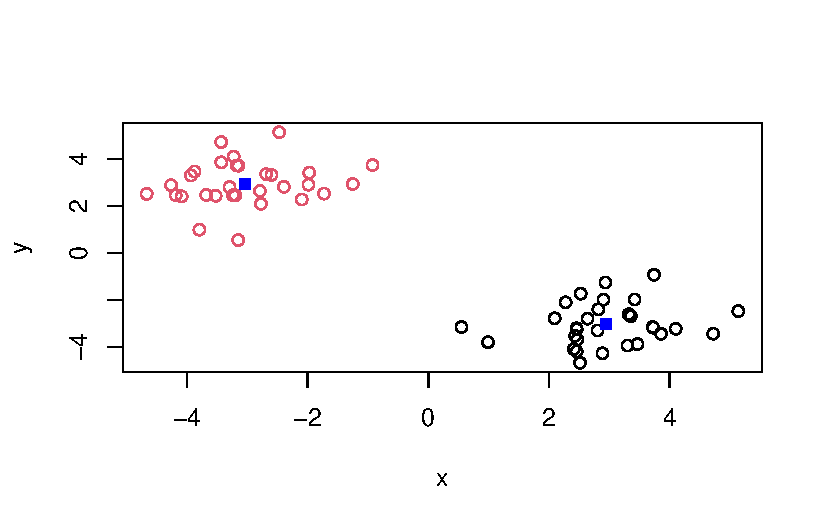
\includegraphics[keepaspectratio]{class07_files/figure-pdf/unnamed-chunk-10-1.pdf}}

\begin{Shaded}
\begin{Highlighting}[]
\FunctionTok{plot}\NormalTok{(z, }\AttributeTok{col=} \FunctionTok{c}\NormalTok{(}\DecValTok{1}\NormalTok{,}\DecValTok{2}\NormalTok{))}
\end{Highlighting}
\end{Shaded}

\pandocbounded{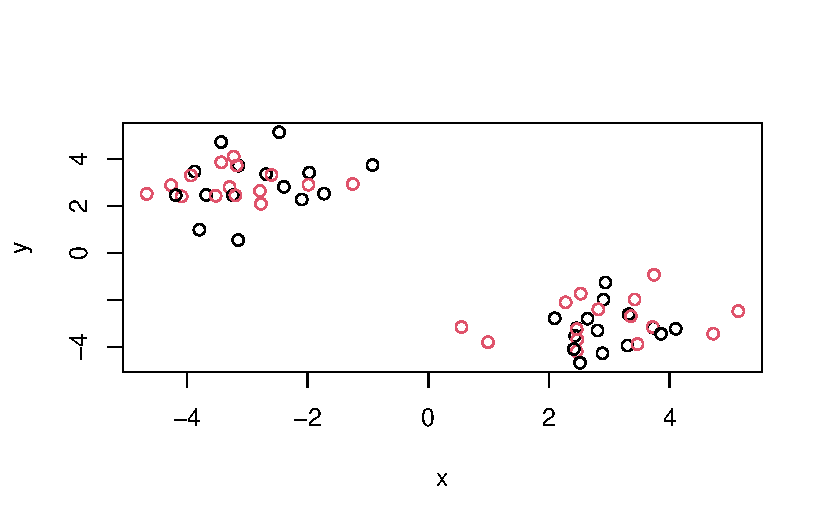
\includegraphics[keepaspectratio]{class07_files/figure-pdf/unnamed-chunk-11-1.pdf}}

\begin{quote}
Q. Run a K-means clustering and plot the results asking for 4 clusters?
\end{quote}

\begin{Shaded}
\begin{Highlighting}[]
\NormalTok{km4 }\OtherTok{\textless{}{-}} \FunctionTok{kmeans}\NormalTok{(z, }\AttributeTok{centers =} \DecValTok{4}\NormalTok{)}
\FunctionTok{plot}\NormalTok{(z, }\AttributeTok{col=}\NormalTok{km4}\SpecialCharTok{$}\NormalTok{cluster)}
\FunctionTok{points}\NormalTok{(km4}\SpecialCharTok{$}\NormalTok{centers, }\AttributeTok{col=} \StringTok{"blue"}\NormalTok{, }\AttributeTok{pch =} \DecValTok{15}\NormalTok{)}
\end{Highlighting}
\end{Shaded}

\pandocbounded{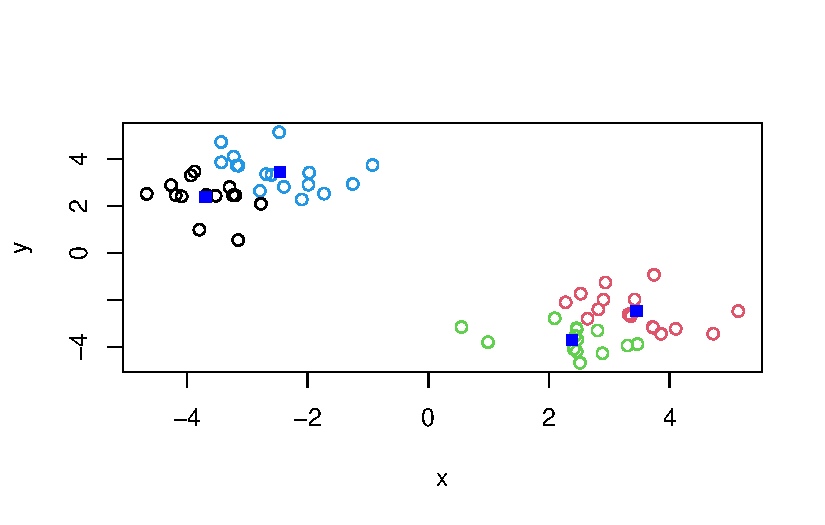
\includegraphics[keepaspectratio]{class07_files/figure-pdf/unnamed-chunk-12-1.pdf}}

\begin{quote}
\textbf{N.B.} You need to tell K-means the number of clusters (i.e.~set
\texttt{centers=2})!!
\end{quote}

One approach is to try different values for \texttt{centers} and then
pick the best\ldots{}

\begin{Shaded}
\begin{Highlighting}[]
\NormalTok{ans }\OtherTok{\textless{}{-}} \ConstantTok{NULL}
\ControlFlowTok{for}\NormalTok{(i }\ControlFlowTok{in} \DecValTok{1}\SpecialCharTok{:}\DecValTok{10}\NormalTok{) \{}
\NormalTok{  km }\OtherTok{\textless{}{-}} \FunctionTok{kmeans}\NormalTok{(z, }\AttributeTok{centers =}\NormalTok{ i)}
\NormalTok{  ans }\OtherTok{\textless{}{-}} \FunctionTok{c}\NormalTok{(ans, km}\SpecialCharTok{$}\NormalTok{tot.withinss)}

\NormalTok{\}}
\FunctionTok{plot}\NormalTok{(ans, }\AttributeTok{type =} \StringTok{"o"}\NormalTok{, }
     \AttributeTok{xlab =} \StringTok{"Number of clusters"}\NormalTok{, }
     \AttributeTok{ylab =} \StringTok{"Total Sum of Squars Distance"}\NormalTok{ )}
\end{Highlighting}
\end{Shaded}

\pandocbounded{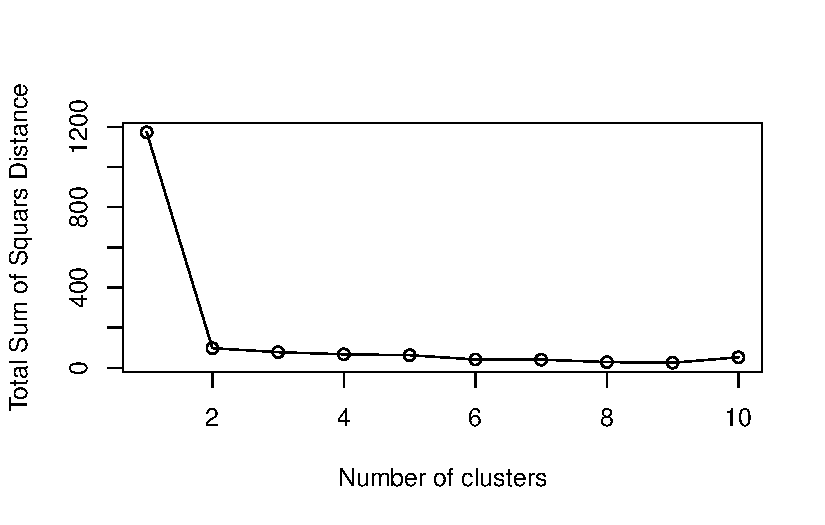
\includegraphics[keepaspectratio]{class07_files/figure-pdf/unnamed-chunk-13-1.pdf}}

\subsection{Hierarchical Clustering}\label{hierarchical-clustering}

The main function in ``base'' R for Hierarchical Clustering is called
\texttt{hclust()}

This function does not take your ``raw'' data for clustering. You must
first build a ``distance matrix'' from your data and pass this as input
to \texttt{hclust()}

\begin{Shaded}
\begin{Highlighting}[]
\NormalTok{d }\OtherTok{\textless{}{-}} \FunctionTok{dist}\NormalTok{(z)}
\NormalTok{hc }\OtherTok{\textless{}{-}} \FunctionTok{hclust}\NormalTok{(d)}
\NormalTok{hc}
\end{Highlighting}
\end{Shaded}

\begin{verbatim}

Call:
hclust(d = d)

Cluster method   : complete 
Distance         : euclidean 
Number of objects: 60 
\end{verbatim}

There is a bespoke \texttt{plot()} method for \texttt{hclust()} result
objects.

\begin{Shaded}
\begin{Highlighting}[]
\FunctionTok{plot}\NormalTok{(hc)}
\FunctionTok{abline}\NormalTok{(}\AttributeTok{h=}\DecValTok{8}\NormalTok{, }\AttributeTok{col=}\StringTok{"red"}\NormalTok{)}
\end{Highlighting}
\end{Shaded}

\pandocbounded{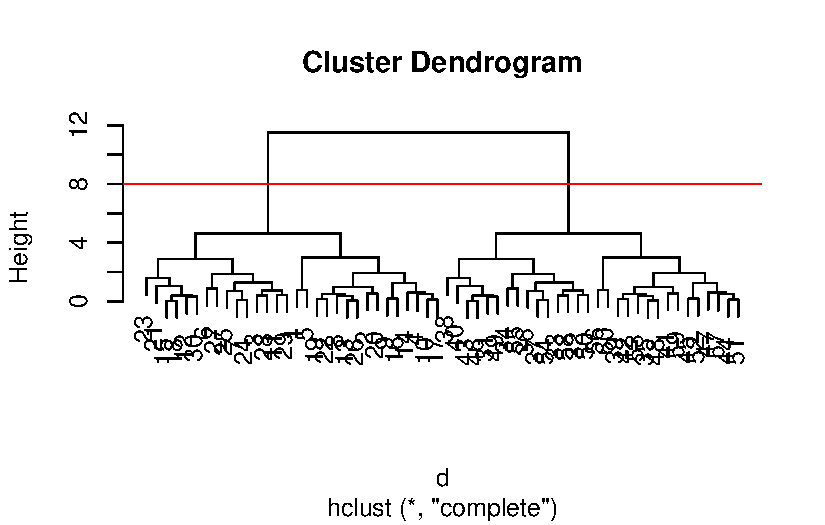
\includegraphics[keepaspectratio]{class07_files/figure-pdf/unnamed-chunk-15-1.pdf}}

Once we have our \texttt{hclust()} object (our ``tree'' of cluster
dendrogram) we can \emph{``cut''} the tree to reveal the clustering
pattern.

\begin{Shaded}
\begin{Highlighting}[]
\FunctionTok{cutree}\NormalTok{(hc, }\AttributeTok{h=}\DecValTok{8}\NormalTok{)}
\end{Highlighting}
\end{Shaded}

\begin{verbatim}
 [1] 1 1 1 1 1 1 1 1 1 1 1 1 1 1 1 1 1 1 1 1 1 1 1 1 1 1 1 1 1 1 2 2 2 2 2 2 2 2
[39] 2 2 2 2 2 2 2 2 2 2 2 2 2 2 2 2 2 2 2 2 2 2
\end{verbatim}

\begin{Shaded}
\begin{Highlighting}[]
\FunctionTok{cutree}\NormalTok{(hc, }\AttributeTok{k=}\DecValTok{4}\NormalTok{)}
\end{Highlighting}
\end{Shaded}

\begin{verbatim}
 [1] 1 1 2 1 1 2 2 1 1 1 2 2 1 1 2 1 1 2 1 1 2 1 2 2 2 1 2 2 2 2 3 3 3 3 4 3 3 3
[39] 4 3 4 4 3 4 4 3 4 4 3 3 4 4 4 3 3 4 4 3 4 4
\end{verbatim}

\begin{Shaded}
\begin{Highlighting}[]
\CommentTok{\#cuts in a way to get 4 groups}
\end{Highlighting}
\end{Shaded}

\begin{quote}
Q. Make a plot of \texttt{z} with your hclust results (i.e.~colored by
cluster membership)
\end{quote}

\begin{Shaded}
\begin{Highlighting}[]
\NormalTok{grps }\OtherTok{\textless{}{-}} \FunctionTok{cutree}\NormalTok{(hc, }\AttributeTok{k=}\DecValTok{2}\NormalTok{)}
\FunctionTok{plot}\NormalTok{(z, }\AttributeTok{col =}\NormalTok{ grps)}
\end{Highlighting}
\end{Shaded}

\pandocbounded{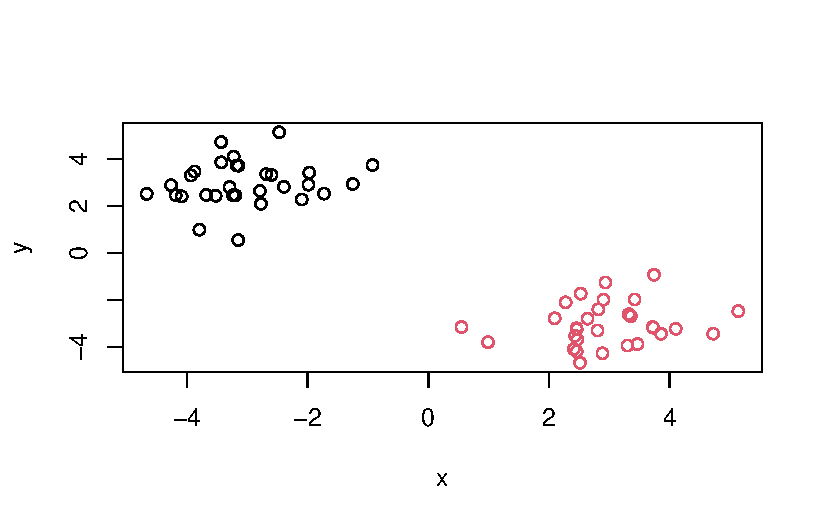
\includegraphics[keepaspectratio]{class07_files/figure-pdf/unnamed-chunk-18-1.pdf}}

\subsection{Principal Component Analysis
(PCA)}\label{principal-component-analysis-pca}

PCA is a dimensionality reduction method that is popular for revealing
patters in complex datasets.

\subsubsection{Analysis of UK food data}\label{analysis-of-uk-food-data}

Let's look at some data on the eating habits of folks from the UK to see
if there are patterns and trends that have the same regions being
distinct frim others.

\subsection{Data Import}\label{data-import}

The data is made available in CSV format so we can use the
\texttt{read.csv()} function for the import to R:

\begin{Shaded}
\begin{Highlighting}[]
\NormalTok{rl }\OtherTok{\textless{}{-}} \StringTok{"https://tinyurl.com/UK{-}foods"}
\NormalTok{x }\OtherTok{\textless{}{-}} \FunctionTok{read.csv}\NormalTok{(rl)}
\end{Highlighting}
\end{Shaded}

\begin{Shaded}
\begin{Highlighting}[]
\FunctionTok{row.names}\NormalTok{(x) }\OtherTok{\textless{}{-}}\NormalTok{ x[, }\DecValTok{1}\NormalTok{]}
\NormalTok{x }\OtherTok{\textless{}{-}}\NormalTok{ x[, }\SpecialCharTok{{-}}\DecValTok{1}\NormalTok{]}
\NormalTok{x}
\end{Highlighting}
\end{Shaded}

\begin{verbatim}
                    England Wales Scotland N.Ireland
Cheese                  105   103      103        66
Carcass_meat            245   227      242       267
Other_meat              685   803      750       586
Fish                    147   160      122        93
Fats_and_oils           193   235      184       209
Sugars                  156   175      147       139
Fresh_potatoes          720   874      566      1033
Fresh_Veg               253   265      171       143
Other_Veg               488   570      418       355
Processed_potatoes      198   203      220       187
Processed_Veg           360   365      337       334
Fresh_fruit            1102  1137      957       674
Cereals                1472  1582     1462      1494
Beverages                57    73       53        47
Soft_drinks            1374  1256     1572      1506
Alcoholic_drinks        375   475      458       135
Confectionery            54    64       62        41
\end{verbatim}

\begin{quote}
\textbf{Q1. How many rows and columns are in your new data frame named
x? What R functions could you use to answer this questions?}
\end{quote}

\begin{Shaded}
\begin{Highlighting}[]
\FunctionTok{nrow}\NormalTok{(x)}
\end{Highlighting}
\end{Shaded}

\begin{verbatim}
[1] 17
\end{verbatim}

\begin{Shaded}
\begin{Highlighting}[]
\FunctionTok{ncol}\NormalTok{(x)}
\end{Highlighting}
\end{Shaded}

\begin{verbatim}
[1] 4
\end{verbatim}

\# Preview the first 6 rows

\begin{Shaded}
\begin{Highlighting}[]
\NormalTok{x }\OtherTok{\textless{}{-}} \FunctionTok{read.csv}\NormalTok{(rl, }\AttributeTok{row.names=}\DecValTok{1}\NormalTok{)}
\FunctionTok{head}\NormalTok{(x)}
\end{Highlighting}
\end{Shaded}

\begin{verbatim}
               England Wales Scotland N.Ireland
Cheese             105   103      103        66
Carcass_meat       245   227      242       267
Other_meat         685   803      750       586
Fish               147   160      122        93
Fats_and_oils      193   235      184       209
Sugars             156   175      147       139
\end{verbatim}

\begin{quote}
\textbf{Q2. Which approach to solving the `row-names problem' mentioned
above do you prefer and why? Is one approach more robust than another
under certain circumstances?}
\end{quote}

I prefer read.csv(url, row.names = 1) because it is cleaner and fixes
the row names during import. It is better when you already know the
first column should be row names. The manual method is useful if the
file was already read incorrectly and needs to be fixed afterward.

\begin{quote}
\textbf{Q3. Changing what optional argument in the above barplot()
function results in the following plot?}
\end{quote}

The optional argument changed is beside, from TRUE to FALSE (or
removed). Setting beside = FALSE produces a stacked barplot instead of
side-by-side bars.

\begin{Shaded}
\begin{Highlighting}[]
\CommentTok{\# Using base R}
\FunctionTok{barplot}\NormalTok{(}\FunctionTok{as.matrix}\NormalTok{(x), }\AttributeTok{beside =}\NormalTok{ T, }\AttributeTok{col =} \FunctionTok{rainbow}\NormalTok{(}\FunctionTok{nrow}\NormalTok{(x)))}
\end{Highlighting}
\end{Shaded}

\pandocbounded{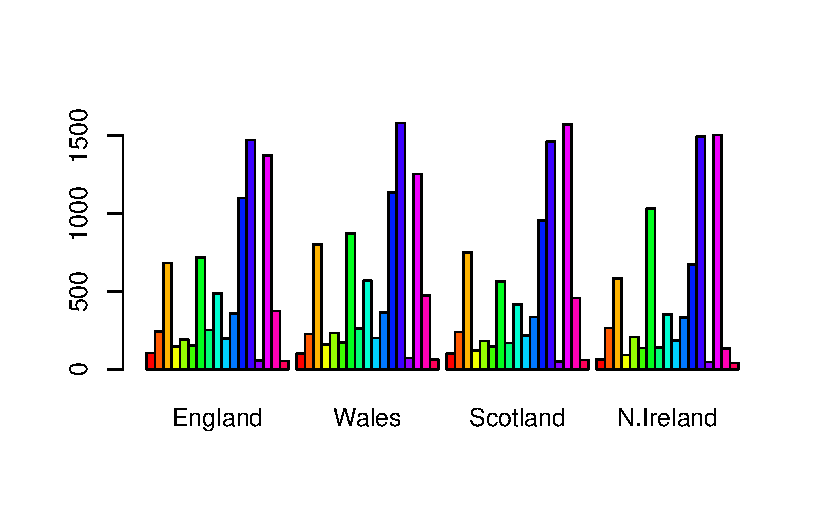
\includegraphics[keepaspectratio]{class07_files/figure-pdf/unnamed-chunk-23-1.pdf}}

\begin{quote}
\textbf{Q4. Changing what optional argument in the above ggplot() code
results in a stacked barplot figure?}
\end{quote}

\begin{Shaded}
\begin{Highlighting}[]
\FunctionTok{library}\NormalTok{(tidyr)}

\CommentTok{\# Convert data to long format for ggplot with \textasciigrave{}pivot\_longer()\textasciigrave{}}
\NormalTok{x\_long }\OtherTok{\textless{}{-}}\NormalTok{ x }\SpecialCharTok{|\textgreater{}} 
\NormalTok{          tibble}\SpecialCharTok{::}\FunctionTok{rownames\_to\_column}\NormalTok{(}\StringTok{"Food"}\NormalTok{) }\SpecialCharTok{|\textgreater{}} 
          \FunctionTok{pivot\_longer}\NormalTok{(}\AttributeTok{cols =} \SpecialCharTok{{-}}\NormalTok{Food, }
                       \AttributeTok{names\_to =} \StringTok{"Country"}\NormalTok{, }
                       \AttributeTok{values\_to =} \StringTok{"Consumption"}\NormalTok{)}

\FunctionTok{dim}\NormalTok{(x\_long)}
\end{Highlighting}
\end{Shaded}

\begin{verbatim}
[1] 68  3
\end{verbatim}

\begin{Shaded}
\begin{Highlighting}[]
\FunctionTok{head}\NormalTok{(x\_long)}
\end{Highlighting}
\end{Shaded}

\begin{verbatim}
# A tibble: 6 x 3
  Food            Country   Consumption
  <chr>           <chr>           <int>
1 "Cheese"        England           105
2 "Cheese"        Wales             103
3 "Cheese"        Scotland          103
4 "Cheese"        N.Ireland          66
5 "Carcass_meat " England           245
6 "Carcass_meat " Wales             227
\end{verbatim}

\begin{Shaded}
\begin{Highlighting}[]
\FunctionTok{library}\NormalTok{(ggplot2)}
\end{Highlighting}
\end{Shaded}

\begin{Shaded}
\begin{Highlighting}[]
\FunctionTok{ggplot}\NormalTok{(x\_long) }\SpecialCharTok{+}
  \FunctionTok{aes}\NormalTok{(}\AttributeTok{x =}\NormalTok{ Country, }\AttributeTok{y =}\NormalTok{ Consumption, }\AttributeTok{fill =}\NormalTok{ Food) }\SpecialCharTok{+}
  \FunctionTok{geom\_col}\NormalTok{(}\AttributeTok{position =} \StringTok{"stack"}\NormalTok{) }\SpecialCharTok{+}
  \FunctionTok{theme\_bw}\NormalTok{()}
\end{Highlighting}
\end{Shaded}

\pandocbounded{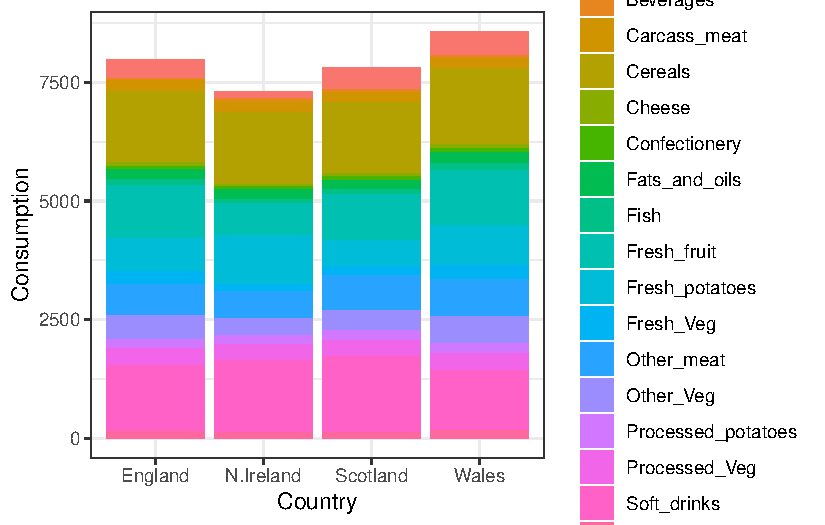
\includegraphics[keepaspectratio]{class07_files/figure-pdf/unnamed-chunk-26-1.pdf}}

The optional argument changed is position from ``dodge'' to ``stack'',
which creates a stacked barplot instead of grouped bars.

\begin{quote}
\textbf{Q5. We can use the pairs() function to generate all pairwise
plots for our countries. Can you make sense of the following code and
resulting figure? What does it mean if a given point lies on the
diagonal for a given plot?}
\end{quote}

The pairs() function creates scatterplots comparing each pair of
countries, where each point represents a food category. If a point lies
on the diagonal, it means the consumption values for that food are equal
(or very similar) between the two countries.

\begin{Shaded}
\begin{Highlighting}[]
\FunctionTok{pairs}\NormalTok{(x, }\AttributeTok{col=}\FunctionTok{rainbow}\NormalTok{(}\FunctionTok{nrow}\NormalTok{(x)), }\AttributeTok{pch=}\DecValTok{16}\NormalTok{)}
\end{Highlighting}
\end{Shaded}

\pandocbounded{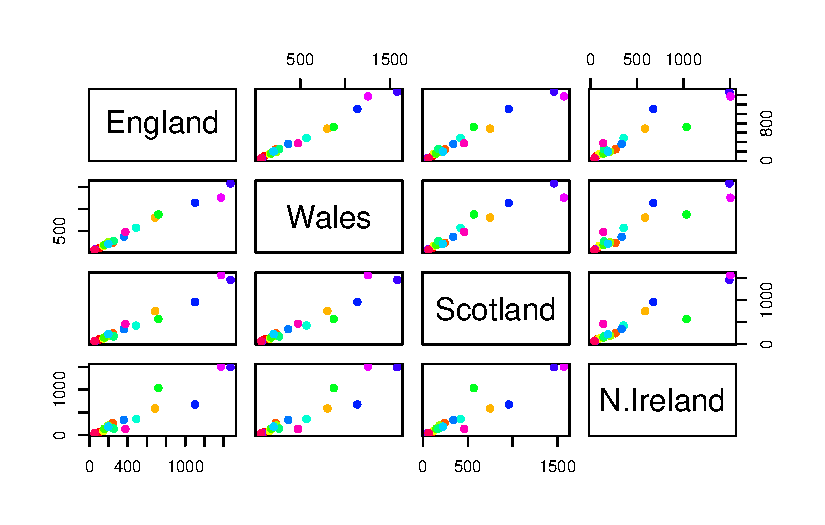
\includegraphics[keepaspectratio]{class07_files/figure-pdf/unnamed-chunk-27-1.pdf}}

\begin{Shaded}
\begin{Highlighting}[]
\FunctionTok{library}\NormalTok{(pheatmap)}

\FunctionTok{pheatmap}\NormalTok{(}\FunctionTok{as.matrix}\NormalTok{(x))}
\end{Highlighting}
\end{Shaded}

\pandocbounded{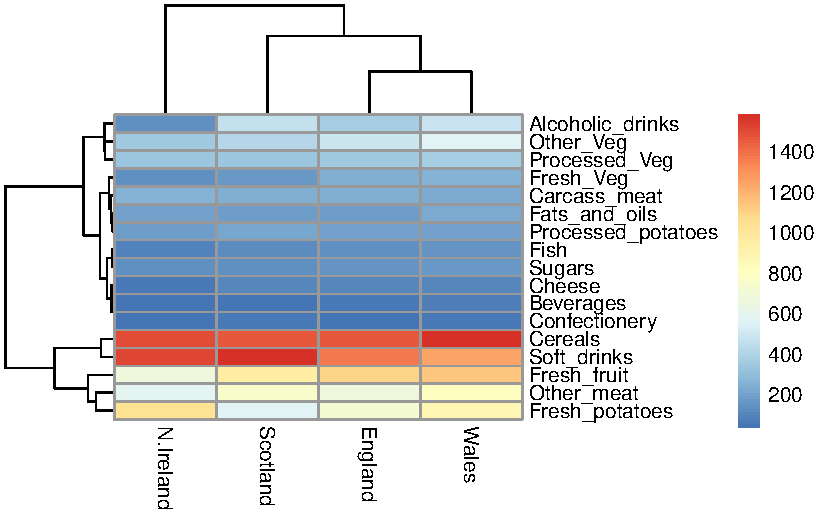
\includegraphics[keepaspectratio]{class07_files/figure-pdf/unnamed-chunk-28-1.pdf}}

\begin{quote}
\textbf{Q6. Based on the pairs and heatmap figures, which countries
cluster together and what does this suggest about their food consumption
patterns? Can you easily tell what the main differences between N.
Ireland and the other countries of the UK in terms of this data-set?}
\end{quote}

England, Wales, and Scotland cluster together, showing similar
consumption patterns. N. Ireland is more distinct. While we can see it
differs overall, the exact food differences are not immediately clear
from these plots alone.

\subsection{Tidy the data}\label{tidy-the-data}

Fix anything that went wrong with import

\subsection{Exporatory analysis}\label{exporatory-analysis}

Make some plots to help make sense of obvious trends\ldots{}

\subsection{PCA to the rescue}\label{pca-to-the-rescue}

The main function in ``base'' R for PCA us called \texttt{prcomp()}.
This function wants the ``observations'' to be rows and the
``variables'' to be columns.

So here we need to take the transpose of ur \texttt{x} input object.

\begin{Shaded}
\begin{Highlighting}[]
\CommentTok{\# Use the prcomp() PCA function }
\NormalTok{pca }\OtherTok{\textless{}{-}} \FunctionTok{prcomp}\NormalTok{( }\FunctionTok{t}\NormalTok{(x) )}
\FunctionTok{summary}\NormalTok{(pca)}
\end{Highlighting}
\end{Shaded}

\begin{verbatim}
Importance of components:
                            PC1      PC2      PC3       PC4
Standard deviation     324.1502 212.7478 73.87622 3.176e-14
Proportion of Variance   0.6744   0.2905  0.03503 0.000e+00
Cumulative Proportion    0.6744   0.9650  1.00000 1.000e+00
\end{verbatim}

so here we need to take the transpose of our \texttt{x} input object

\begin{Shaded}
\begin{Highlighting}[]
\NormalTok{pca }\OtherTok{\textless{}{-}} \FunctionTok{prcomp}\NormalTok{( }\FunctionTok{t}\NormalTok{(x) )}
\FunctionTok{summary}\NormalTok{(pca)}
\end{Highlighting}
\end{Shaded}

\begin{verbatim}
Importance of components:
                            PC1      PC2      PC3       PC4
Standard deviation     324.1502 212.7478 73.87622 3.176e-14
Proportion of Variance   0.6744   0.2905  0.03503 0.000e+00
Cumulative Proportion    0.6744   0.9650  1.00000 1.000e+00
\end{verbatim}

The returned \texttt{pca} object has components we can use to make our
main result figures:

\begin{Shaded}
\begin{Highlighting}[]
\FunctionTok{attributes}\NormalTok{(pca)}
\end{Highlighting}
\end{Shaded}

\begin{verbatim}
$names
[1] "sdev"     "rotation" "center"   "scale"    "x"       

$class
[1] "prcomp"
\end{verbatim}

The main result figure from this analysis is called a \textbf{``score
plot''} (a.k.a an ``ordination plot'', ``PC plot'' or simply ``PC1 vs
PC2 plot'').

This plot shows how samples (in this case countries) relate to each
other along our new PC axis.

This is our new ``reduced-dimensional space''. In this case 2
dimensions, PC1 and PC2, that capture most of the variance in the
original 17 dimensional data-set.

\begin{Shaded}
\begin{Highlighting}[]
\FunctionTok{library}\NormalTok{(ggplot2)}

\FunctionTok{ggplot}\NormalTok{(pca}\SpecialCharTok{$}\NormalTok{x) }\SpecialCharTok{+}
  \FunctionTok{aes}\NormalTok{(PC1, PC2) }\SpecialCharTok{+} 
  \FunctionTok{geom\_point}\NormalTok{()}
\end{Highlighting}
\end{Shaded}

\pandocbounded{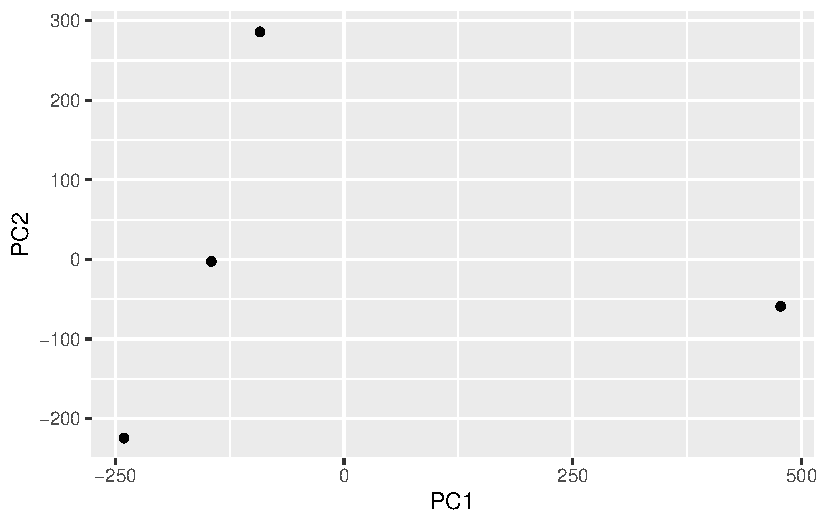
\includegraphics[keepaspectratio]{class07_files/figure-pdf/unnamed-chunk-32-1.pdf}}

\begin{Shaded}
\begin{Highlighting}[]
\FunctionTok{ggplot}\NormalTok{(pca}\SpecialCharTok{$}\NormalTok{rotation) }\SpecialCharTok{+}
  \FunctionTok{aes}\NormalTok{(PC1, }\FunctionTok{row.names}\NormalTok{(pca}\SpecialCharTok{$}\NormalTok{rotation)) }\SpecialCharTok{+}
  \FunctionTok{geom\_col}\NormalTok{()}
\end{Highlighting}
\end{Shaded}

\pandocbounded{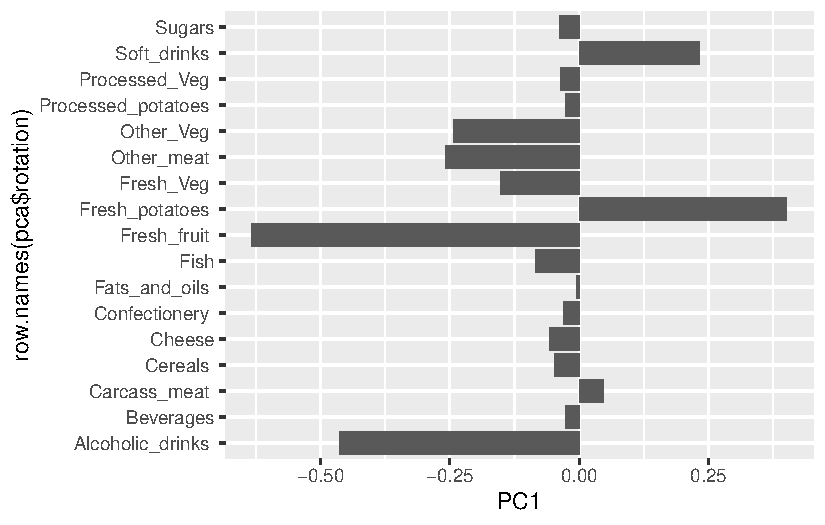
\includegraphics[keepaspectratio]{class07_files/figure-pdf/unnamed-chunk-33-1.pdf}}

\begin{Shaded}
\begin{Highlighting}[]
\NormalTok{mycols }\OtherTok{\textless{}{-}} \FunctionTok{c}\NormalTok{(}\StringTok{"orange"}\NormalTok{, }\StringTok{"red"}\NormalTok{, }\StringTok{"blue"}\NormalTok{, }\StringTok{"darkgreen"}\NormalTok{)}

\FunctionTok{ggplot}\NormalTok{(pca}\SpecialCharTok{$}\NormalTok{x) }\SpecialCharTok{+}
  \FunctionTok{aes}\NormalTok{(PC1, PC2) }\SpecialCharTok{+} 
  \FunctionTok{geom\_point}\NormalTok{(}\AttributeTok{col=}\NormalTok{mycols)}
\end{Highlighting}
\end{Shaded}

\pandocbounded{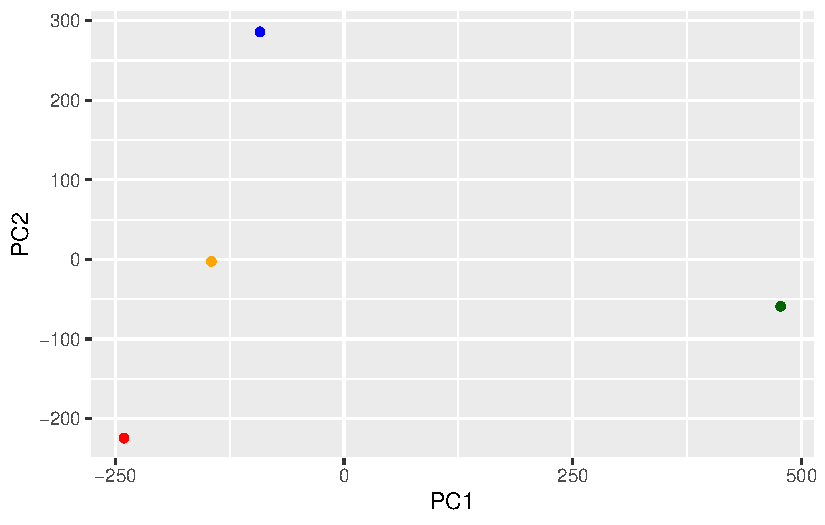
\includegraphics[keepaspectratio]{class07_files/figure-pdf/unnamed-chunk-34-1.pdf}}

\begin{Shaded}
\begin{Highlighting}[]
\FunctionTok{ggplot}\NormalTok{(pca}\SpecialCharTok{$}\NormalTok{x) }\SpecialCharTok{+}
  \FunctionTok{aes}\NormalTok{(PC1, PC2, }\AttributeTok{label=}\FunctionTok{row.names}\NormalTok{(pca}\SpecialCharTok{$}\NormalTok{x)) }\SpecialCharTok{+} 
  \FunctionTok{geom\_point}\NormalTok{(}\AttributeTok{col=}\NormalTok{mycols) }\SpecialCharTok{+}
  \FunctionTok{geom\_text}\NormalTok{(}\AttributeTok{size=}\DecValTok{3}\NormalTok{, }\AttributeTok{vjust=}\DecValTok{2}\NormalTok{, }\AttributeTok{col=}\NormalTok{mycols)}
\end{Highlighting}
\end{Shaded}

\pandocbounded{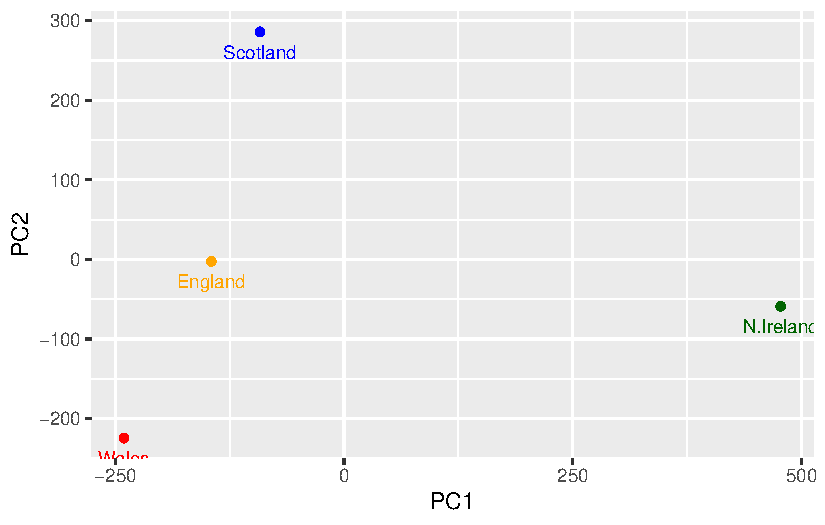
\includegraphics[keepaspectratio]{class07_files/figure-pdf/unnamed-chunk-35-1.pdf}}

\begin{quote}
\textbf{Q7. Complete the code below to generate a plot of PC1 vs PC2.
The second line adds text labels over the data points.}
\end{quote}

\begin{Shaded}
\begin{Highlighting}[]
\CommentTok{\# Create a data frame for plotting}
\NormalTok{df }\OtherTok{\textless{}{-}} \FunctionTok{as.data.frame}\NormalTok{(pca}\SpecialCharTok{$}\NormalTok{x)}
\NormalTok{df}\SpecialCharTok{$}\NormalTok{Country }\OtherTok{\textless{}{-}} \FunctionTok{rownames}\NormalTok{(df)}

\CommentTok{\# Plot PC1 vs PC2 with ggplot}
\FunctionTok{ggplot}\NormalTok{(pca}\SpecialCharTok{$}\NormalTok{x) }\SpecialCharTok{+}
  \FunctionTok{aes}\NormalTok{(}\AttributeTok{x =}\NormalTok{ PC1, }\AttributeTok{y =}\NormalTok{ PC2, }\AttributeTok{label =} \FunctionTok{rownames}\NormalTok{(pca}\SpecialCharTok{$}\NormalTok{x)) }\SpecialCharTok{+}
  \FunctionTok{geom\_point}\NormalTok{(}\AttributeTok{size =} \DecValTok{3}\NormalTok{) }\SpecialCharTok{+}
  \FunctionTok{geom\_text}\NormalTok{(}\AttributeTok{vjust =} \SpecialCharTok{{-}}\FloatTok{0.5}\NormalTok{) }\SpecialCharTok{+}
  \FunctionTok{xlim}\NormalTok{(}\SpecialCharTok{{-}}\DecValTok{270}\NormalTok{, }\DecValTok{500}\NormalTok{) }\SpecialCharTok{+}
  \FunctionTok{xlab}\NormalTok{(}\StringTok{"PC1"}\NormalTok{) }\SpecialCharTok{+}
  \FunctionTok{ylab}\NormalTok{(}\StringTok{"PC2"}\NormalTok{) }\SpecialCharTok{+}
  \FunctionTok{theme\_bw}\NormalTok{()}
\end{Highlighting}
\end{Shaded}

\pandocbounded{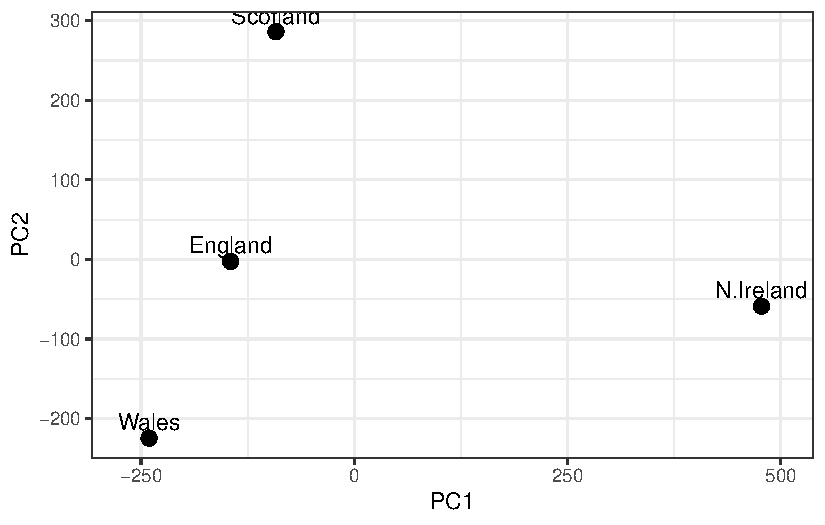
\includegraphics[keepaspectratio]{class07_files/figure-pdf/unnamed-chunk-36-1.pdf}}

\begin{quote}
\textbf{Q8. Customize your plot so that the colors of the country names
match the colors in our UK and Ireland map and table at start of this
document.}
\end{quote}

\begin{Shaded}
\begin{Highlighting}[]
\FunctionTok{ggplot}\NormalTok{(pca}\SpecialCharTok{$}\NormalTok{x) }\SpecialCharTok{+}
  \FunctionTok{aes}\NormalTok{(}\AttributeTok{x =}\NormalTok{ PC1, }\AttributeTok{y =}\NormalTok{ PC2, }\AttributeTok{label =} \FunctionTok{rownames}\NormalTok{(pca}\SpecialCharTok{$}\NormalTok{x), }\AttributeTok{color =} \FunctionTok{rownames}\NormalTok{(pca}\SpecialCharTok{$}\NormalTok{x)) }\SpecialCharTok{+}
  \FunctionTok{geom\_point}\NormalTok{(}\AttributeTok{size =} \DecValTok{3}\NormalTok{) }\SpecialCharTok{+}
  \FunctionTok{geom\_text}\NormalTok{(}\AttributeTok{vjust =} \SpecialCharTok{{-}}\FloatTok{0.5}\NormalTok{) }\SpecialCharTok{+}
  \FunctionTok{scale\_color\_manual}\NormalTok{(}\AttributeTok{values =} \FunctionTok{c}\NormalTok{(}
    \StringTok{"England"} \OtherTok{=} \StringTok{"orange"}\NormalTok{,}
    \StringTok{"Wales"} \OtherTok{=} \StringTok{"red"}\NormalTok{,}
    \StringTok{"Scotland"} \OtherTok{=} \StringTok{"blue"}\NormalTok{,}
    \StringTok{"N.Ireland"} \OtherTok{=} \StringTok{"darkgreen"}
\NormalTok{  )) }\SpecialCharTok{+}
  \FunctionTok{xlim}\NormalTok{(}\SpecialCharTok{{-}}\DecValTok{270}\NormalTok{, }\DecValTok{500}\NormalTok{) }\SpecialCharTok{+}
  \FunctionTok{xlab}\NormalTok{(}\StringTok{"PC1"}\NormalTok{) }\SpecialCharTok{+}
  \FunctionTok{ylab}\NormalTok{(}\StringTok{"PC2"}\NormalTok{) }\SpecialCharTok{+}
  \FunctionTok{theme\_bw}\NormalTok{()}
\end{Highlighting}
\end{Shaded}

\pandocbounded{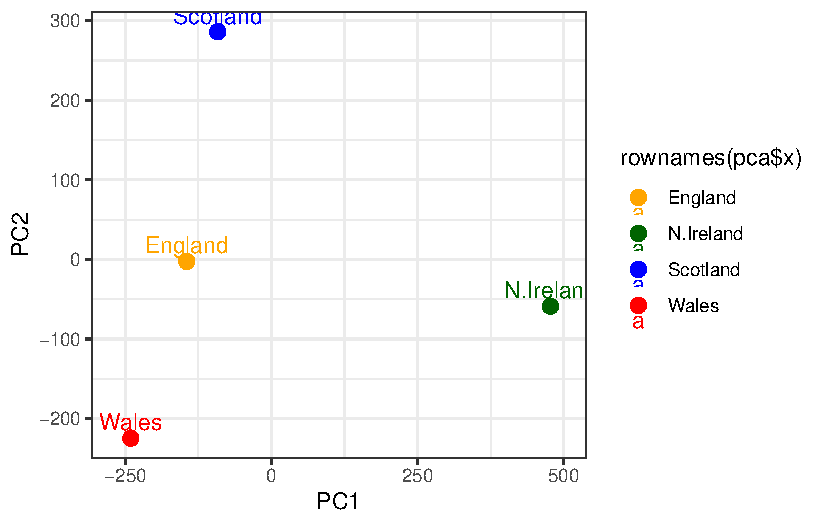
\includegraphics[keepaspectratio]{class07_files/figure-pdf/unnamed-chunk-37-1.pdf}}

\begin{quote}
\textbf{Q9. Generate a similar `loadings plot' for PC2. What two food
groups feature prominantely and what does PC2 maninly tell us about?}
\end{quote}

\begin{Shaded}
\begin{Highlighting}[]
\FunctionTok{ggplot}\NormalTok{(pca}\SpecialCharTok{$}\NormalTok{rotation) }\SpecialCharTok{+}
  \FunctionTok{aes}\NormalTok{(}\AttributeTok{x =}\NormalTok{ PC2, }\AttributeTok{y =} \FunctionTok{reorder}\NormalTok{(}\FunctionTok{rownames}\NormalTok{(pca}\SpecialCharTok{$}\NormalTok{rotation), PC2)) }\SpecialCharTok{+}
  \FunctionTok{geom\_col}\NormalTok{(}\AttributeTok{fill =} \StringTok{"steelblue"}\NormalTok{) }\SpecialCharTok{+}
  \FunctionTok{xlab}\NormalTok{(}\StringTok{"PC2 Loading Score"}\NormalTok{) }\SpecialCharTok{+}
  \FunctionTok{ylab}\NormalTok{(}\StringTok{""}\NormalTok{) }\SpecialCharTok{+}
  \FunctionTok{theme\_bw}\NormalTok{() }\SpecialCharTok{+}
  \FunctionTok{theme}\NormalTok{(}\AttributeTok{axis.text.y =} \FunctionTok{element\_text}\NormalTok{(}\AttributeTok{size =} \DecValTok{9}\NormalTok{))}
\end{Highlighting}
\end{Shaded}

\pandocbounded{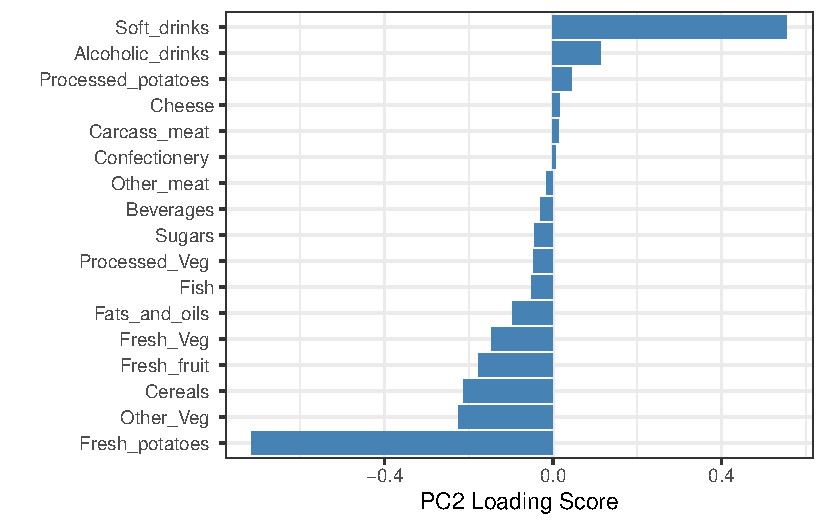
\includegraphics[keepaspectratio]{class07_files/figure-pdf/unnamed-chunk-38-1.pdf}}

Fresh\_veg and Fresh\_fruit (strong loadings on one side) vs
Soft\_drinks (and sometimes Processed foods) on the opposite side. PC2
mainly represents a contrast between healthier fresh foods (fruits \&
vegetables) and less healthy / processed items (like soft drinks).

The score plot shows how samples are positioned along principal
components, while the loading plot shows which variables influence those
components. The loadings explain why samples appear where they do in the
score plot.

\begin{quote}
\textbf{Q10. How many genes and samples are in this data set? How many
PCs do you think it will take to have a useful overview of this data set
(see below)?}
\end{quote}

\begin{Shaded}
\begin{Highlighting}[]
\NormalTok{url2 }\OtherTok{\textless{}{-}} \StringTok{"https://tinyurl.com/expression{-}CSV"}
\NormalTok{rna.data }\OtherTok{\textless{}{-}} \FunctionTok{read.csv}\NormalTok{(url2, }\AttributeTok{row.names=}\DecValTok{1}\NormalTok{)}
\FunctionTok{head}\NormalTok{(rna.data)}
\end{Highlighting}
\end{Shaded}

\begin{verbatim}
       wt1 wt2  wt3  wt4 wt5 ko1 ko2 ko3 ko4 ko5
gene1  439 458  408  429 420  90  88  86  90  93
gene2  219 200  204  210 187 427 423 434 433 426
gene3 1006 989 1030 1017 973 252 237 238 226 210
gene4  783 792  829  856 760 849 856 835 885 894
gene5  181 249  204  244 225 277 305 272 270 279
gene6  460 502  491  491 493 612 594 577 618 638
\end{verbatim}

\begin{Shaded}
\begin{Highlighting}[]
\DocumentationTok{\#\# Again we have to take the transpose of our data }
\NormalTok{pca }\OtherTok{\textless{}{-}} \FunctionTok{prcomp}\NormalTok{(}\FunctionTok{t}\NormalTok{(rna.data), }\AttributeTok{scale=}\ConstantTok{TRUE}\NormalTok{)}

\CommentTok{\# Create data frame for plotting}
\NormalTok{df }\OtherTok{\textless{}{-}} \FunctionTok{as.data.frame}\NormalTok{(pca}\SpecialCharTok{$}\NormalTok{x)}
\NormalTok{df}\SpecialCharTok{$}\NormalTok{Sample }\OtherTok{\textless{}{-}} \FunctionTok{rownames}\NormalTok{(df)}

\DocumentationTok{\#\# Plot with ggplot}
\FunctionTok{ggplot}\NormalTok{(df) }\SpecialCharTok{+}
  \FunctionTok{aes}\NormalTok{(}\AttributeTok{x =}\NormalTok{ PC1, }\AttributeTok{y =}\NormalTok{ PC2, }\AttributeTok{label =}\NormalTok{ Sample) }\SpecialCharTok{+}
  \FunctionTok{geom\_point}\NormalTok{(}\AttributeTok{size =} \DecValTok{3}\NormalTok{) }\SpecialCharTok{+}
  \FunctionTok{geom\_text}\NormalTok{(}\AttributeTok{vjust =} \SpecialCharTok{{-}}\FloatTok{0.5}\NormalTok{, }\AttributeTok{size =} \DecValTok{3}\NormalTok{) }\SpecialCharTok{+}
  \FunctionTok{xlab}\NormalTok{(}\StringTok{"PC1"}\NormalTok{) }\SpecialCharTok{+}
  \FunctionTok{ylab}\NormalTok{(}\StringTok{"PC2"}\NormalTok{) }\SpecialCharTok{+}
  \FunctionTok{theme\_bw}\NormalTok{()}
\end{Highlighting}
\end{Shaded}

\pandocbounded{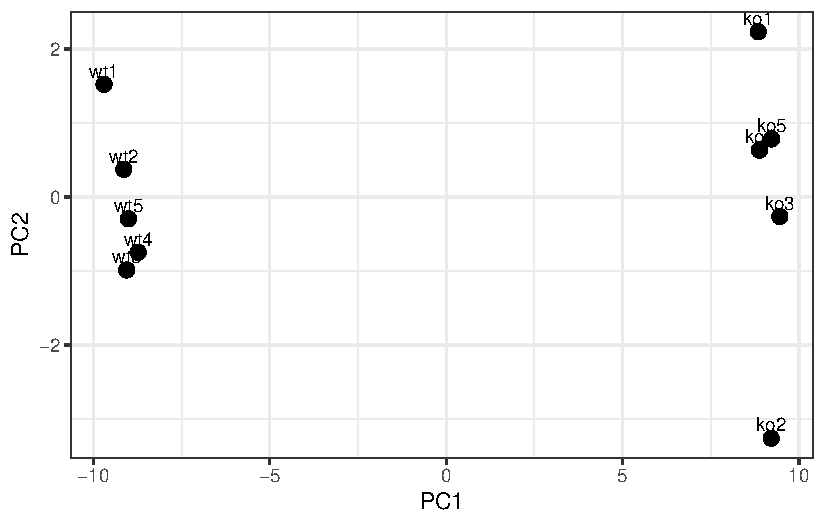
\includegraphics[keepaspectratio]{class07_files/figure-pdf/unnamed-chunk-40-1.pdf}}

The dataset has 100 genes and 10 samples. About 1--2 principal
components are sufficient, since PC1 explains \textasciitilde92.6\% of
the variance and PC2 adds a small amount more.




\end{document}
